\chapter{おわりに}
\section{関連研究}
\subsection*{組込みシステム向けデバッガソフトウェア}
組込みシステム向けデバッガソフトウェアには,機能の1つとしてトレースログを可視化する機能が含まれている場合がある.
組込みシステム向けデバッガソフトウェアとは,ICE(In-Circuit Emulator)やJTAGエミュレータなどの,組込みシステム向けデバッガに付属するデバッグ用のソフトウェアである.
組込みシステム向けデバッガとは,ターゲットシステム上で動くプログラムをホストシステム上でデバッグを行えるようにするために,ターゲットCPUにアクセスする手段を提供する装置を指す.

組込みシステム向けデバッガソフトウェアとしては,京都マイクロコンピュータ株式会社のPARTNER\cite{PARTNER-JET}や,株式会社ソフィアシステムズのWatchPoint\cite{watchpoint}などがあり,それぞれ,イベントトラッカー,OSアナライザというトレースログを可視化する機能を提供している.
図\ref{fig:PARTNER-JET}に,イベントトラッカーのスクリーンショットを,図\ref{fig:watchpoint}にOSアナライザのスクリーンショットを示す.

これら組込みシステム向けデバッガソフトウェアの一機能としての可視化ツールは,その性質からターゲットとなるOSやプロセッサが限定される.
これは,組込みシステム向けデバッガは,通常,ターゲットとなるプロセッサが限られており,デバッガソフトウェアが対応するOSも限られているからである.
また,可視化表示したい情報も提供されているものに限られるなど,可視化ツールとしては汎用性,拡張性に乏しい.

\begin{figure}
\begin{center}
\includegraphics[height=6cm]{PARTNER-JET.eps}
\caption{PARTNER イベントトラッカー}
\label{fig:PARTNER-JET}
\end{center}
\end{figure}

\begin{figure}
\begin{center}
\includegraphics[height=4cm]{watchpoint.eps}
\caption{WatchPoint OSアナライザ}
\label{fig:watchpoint}
\end{center}
\end{figure}

\subsection*{組込みOS向けの統合開発環境}

QNX Software Systems社は,自社の組込みリアルタイムオペレーティングシステムQNXの統合開発環境としてQNX Momenticsを販売している.QNX Momenticsにはシステムプロファイラとして,システムコールや割込み,スレッド状態やメッセージなどを可視化するQNX System Profiler\cite{QNXMomentics}という機能を提供している.図\ref{fig:QNXSystemProfiler}にQNX System Profilerのスクリーンショットを示す.

また,イーソル株式会社はT-Kernel/$\mu$ITRONベースシステムの統合開発環境としてeBinder\cite{eBinder}を販売している.eBinderにはイベントログ取得・解析ツールとしてEvenTrekが付属しており,システムコール,割込み,タスクスイッチ,タスク状態遷移などを可視化することができる.図\ref{fig:EvenTrek}にEvenTrekのスクリーンショットを示す.

このように,商用の組込みOS向けの統合開発環境にはOSの実行履歴を可視化表示する機能が搭載されている場合がある.しかしながら,これらは,各ベンダーが自社OSの競争力を高めるために提供しているものであり,当然ながら可視化表示に対応するOSは自社提供のものに限られている.
また,可視化表示する情報も提供するものに限られており,表示のカスタマイズ機能もそれほど自由度は高くはない.

\begin{figure}
\begin{center}
\includegraphics[height=6cm]{QNXSystemProfiler.eps}
\caption{QNXSystemProfiler}
\label{fig:QNXSystemProfiler}
\end{center}
\end{figure}

\begin{figure}
\begin{center}
\includegraphics[height=6cm]{EvenTrek.eps}
\caption{eBinder EvenTrek}
\label{fig:EvenTrek}
\end{center}
\end{figure}

\subsection*{Unix系OSのトレースログプロファイラ}

Unix系OSでは,これまでに,パフォーマンスチューニングや障害解析を目的として,カーネルの実行トレースを取得するソフトウェアがいくつか開発されている.
ここでは,単にこれをトレースツールと呼称する.

Linux用のトレースツールとしてはLKST\cite{LKST},SystemTap\cite{SystemTap},LTTng\cite{LTTng}などがあり,Solaris用にはDtrace\cite{Dtrace}がある.
これらトレースツールが提供する主な機能は,カーネル内にフックを仕込みカーネル内部状態をユーザー空間に通知する機能と通知をログとして記録する機能である.

これらのトレースツールは,ログを分析,提示する,専用のプロファイラツールを提供している場合が多い.
たとえば,LTTngにはLTTV\cite{LTTV}が,DTraceにはChime\cite{Chime}が,プロファイラツールとして提供されている.
図\ref{fig:LTTV}にLTTVのスクリーンショットを,図\ref{fig:Chime}にChimeのスクリーンショットを示す.

これら,プロファイラツールは,主に,カーネルの内部状態を統計情報として出力することにより,ボトルネックを探したり,障害の要因を探る目的で使用されるが,ソフトウェアのデバッグを目的に使用することもできる.
DTraceなどはログ出力のためのカーネルフックポイントを独自のスクリプト言語を用いて制御できるなど,任意の情報をソフトウェアの実行から取得することができる.
しかしながら,取得したログを任意の図形で可視化する手段は提供されておらず,テキスト形式での確認となる.
また,可視化表示する際のログの形式は,そのOSのトレースツールが出力する形式に依存するため,他のOSのトレースを可視化することはできない.

\begin{figure}
\begin{center}
\includegraphics[height=6cm]{LTTV.eps}
\caption{LTTV}
\label{fig:LTTV}
\end{center}
\end{figure}

\begin{figure}
\begin{center}
\includegraphics[height=6cm]{Chime.eps}
\caption{Chime}
\label{fig:Chime}
\end{center}
\end{figure}

\subsection*{波形表示ツールの流用}
任意のOS,アプリケーションのトレースログを可視化表示する手段として,波形表示ツールを流用する方法がある.
波形表示ツールとは,Verilog等のデジタル回路設計用論理シミュレータの実行ログを波形で表示するソフトウェアのことを指す.

デジタル回路設計用論理シミュレータの実行ログには,VCD(Value Change Dump)形式というオープンなファイルフォーマットが存在する.
そのため,任意のログをVCD形式として出力することにより,これらのツールで可視化表示することが可能になる.
図\ref{fig:GTKWave}に,VCD形式のログの可視化に対応した波形表示ツールGTKWaveのスクリーンショットを示す.

波形表示ツールを流用する方法では,任意のログをオープンフォーマットなファイル形式に変換することによりログの形式に依存せずに利用できる反面,表示能力に乏しく,複雑な可視化表現は難しいという問題がある.

\begin{figure}
\begin{center}
\includegraphics[height=6cm]{GTKWave.eps}
\caption{GTKWave}
\label{fig:GTKWave}
\end{center}
\end{figure}

\section{まとめ}
本OJLでは、トレースログ可視化ツールであるTLVの開発を継続して行ない、
TLVに対して機能追加とリファクタリングを行なった。

TLVを開発された背景として,組込みシステムにおいてもマルチコアプロセッサ
の利用が進んでおり,それに伴い従来のデバッグ方法が有効でなくなってきた
ことを述べた.これは,マルチコアプロセッサが各コアで並列処理を行うため,
プログラムの挙動が非決定的になり,バグの再現が保証されず,従来のブレー
クポイントによるステップ実行ではバグを確実に捕らえることができないから
である.

一方,マルチコアプロセッサ環境におけるデバッグで有効な方法として,実行
中にデバッグを行うのではなく,実行後にトレースログを解析する手法がある
.そして,開発者が直接トレースログを扱うのは効率が悪く,ト
レースログの解析を支援するツールが要求されており,その1つとして可視化表
示ツールがある.

既存のトレースログ可視化ツールは,標準化されたトレースログを扱っていな
いため,利用できるトレースログの形式が限られており,汎用性に乏しい。
また,可視化表示項目が提供されているものに限られ,変更や追加
を行う仕組みも提供されておらず,拡張性に乏しい。

そこで後藤ら\cite{goto,ipsj}によって、汎用性と拡張性を備えたトレースロ
グ可視化ツールTLVが開発された。TLV内部でトレースログを抽象的に扱えるよ
う、トレースログを一般化した標準形式トレースログを定め、任意の形式のト
レースログを標準形式トレースログに変換する仕組みを変換ルールとして形式
化した。トレースログの可視化表現を指示する仕組みを抽象化し、可視化ルー
ルとして形式化した。TLVでは、変換ルールと可視化ルールを外部ファイルとし
て与えることで、汎用性と拡張性を実現している。

本OJLでは、TLVのリリースを複数回行ない、要求の収集を行なった。
収集した要求のうち``CPU利用率表
示などの複雑な可視化の実現''と``TLVの高速化''に対する要求が強かったため、
これらの実現を行なった。

複雑な可視化を行なうための機能追加を行なった。変換・可視化を外部プロセ
スで行なえるようすることで、任意の言語で変換ルール・可視化ルールを記述
できるようにした。変換ルール・可視化ルールの互換性を保つように機能追加
を行ったため、従来のルールと混在させて利用することも可能である。
実際にCPU利用率の可視化を行ない、有用性を確認した。

TLVの高速化を行なうためには、
標準形式トレースログへの変換と図形データの生成を高速化する必要がある。
その際、変換処理と図形データに関するソースコードが複雑化している点が障害となる。
そこで、複雑化している原因の調査を行ない、その原因を改善する
リファクタリング方針の決定を行なった。

\section{今後の課題}
\subsection*{変換・可視化の高速化}
TLVの変換・可視化の高速化を行なう必要がある。

\ref{ch:ref}章で述べたリファクタリング方針に従い、
リファクタリングの実施を行なう必要がある。
その後、プロファイラ等を用いて、ボトルネックの特定を行ない、
ボトルネックを改善し、変換・可視化の高速化を行なう必要がある。

\subsection*{TLVの応答性の向上}
TLVの応答性を向上させる必要がある。

現在、大量のトレースログを可視化した際、スクロールバーの応答性が鈍いた
め、操作性が悪い。スクロールバー以外の可視化範囲の変更方法を提供するこ
とで、改善する必要がある。

%% \subsection*{要求の実装}
%% TLVに対して寄せられている要求を実装する必要がある。
